\documentclass[a4paper, 12pt]{report}
\usepackage[utf8]{inputenc}
\usepackage[french]{babel}
\usepackage[pdftex]{graphicx}
\usepackage{fancyhdr}
\usepackage{algorithm}
\usepackage{algorithmic}
\usepackage{cite}
\usepackage{microtype}
\usepackage{makecell}
\usepackage{hyperref}
\usepackage{tikz}
\usepackage{qtree}
\usepackage{newfloat}
\usepackage{moreverb}
\usepackage{hyperref}
%\usepackage[dvips]{hyperref}
\hypersetup{
colorlinks=true,
linkcolor=red,           
}
\setcounter{tocdepth}{5} %pour l'apparition dans la table des matières des susubsections
%\setcounter{secnumdepth}{5}%pour la numérotation dans le corps du document des susubsections

%\pagestyle{fancy}
%olsr
%parler d'esp32
%choix environnement 
%idf base sur frrrtos
%fenetre esp mesh
\newcommand{\esp}{\textsc{esp32}}
\newcommand{\espmesh}{\textsc{esp-mesh}}
\newcommand{\mac}{\textsc{mac}}
\newcommand{\rssi}{\textsc{rssi}}
\newcommand{\mesh}{\textsc{mesh}}
\newcommand{\espnow}{\textsc{esp now}}
\newcommand{\wifi}{Wi-Fi}
\newcommand{\aodv}{\textsc{aodv}}

\DeclareFloatingEnvironment[fileext=lod]{diagram}

\begin{document}
%\pagenumbering{roman}

\begin{titlepage}
\begin{center}

{\Large Université de Mons}\\[1ex]
{\Large Faculté des sciences}\\[1ex]
{\Large Département d'Informatique}\\[1ex]
{\Large Service de réseaux et télécommunications}\\[2.5cm]

\newcommand{\HRule}{\rule{\linewidth}{0.3mm}}
% Title
\HRule \\[0.3cm]
{ \LARGE \bfseries Réseau Wi-Fi multi-sauts sur plateforme ESP \\[0.3cm]}
{ \LARGE \bfseries Rapport de projet \\[0.1cm]}
\HRule \\[1.5cm]

% Author and supervisor
\begin{minipage}[t]{0.45\textwidth}
\begin{flushleft} \large
\emph{Directeur:}\\
Bruno \textsc{Quoitin}
\end{flushleft}
\end{minipage}
\begin{minipage}[t]{0.45\textwidth}
\begin{flushright} \large
\emph{Auteur:} \\
Arnaud \textsc{Palgen}
\end{flushright}
\end{minipage}\\[2ex]

\vfill

% Bottom of the page
\begin{center}
\begin{tabular}[t]{c c c}

\includegraphics[height=1.5cm]{images/logoumons.jpg} &
\hspace{0.3cm} &

\includegraphics[height=1.5cm]{images/logofs.jpg}
\end{tabular}
\end{center}~\\
 
{\large Année académique 2019-2020}

\end{center}
\end{titlepage}


\chapter*{Introduction}
    L'objectif du projet est de concevoir un réseau \wifi\ multi-sauts composé 
    de micro-contrôleurs \wifi. L'\esp\ d'Espressif sera utilisé en raison de 
    son très faible coût.\\
    Le projet tiendra compte de la consommation énergétique des noeuds du 
    réseau du fait qu'ils soient alimentés par batterie.\\
    Le réseau ainsi créé sera testé pour en évaluer sa performance et ses fonctionnalités. 
    Il sera également étudié pour notamment analyser la durée du vie du réseau 
    sur batterie, analyser la longueur des chemins établis, etc.

\tableofcontents
\newpage

\chapter{Etat de l'Art}
\section{Présentation de l'ESP}
    L'\esp\ est un système embarqué développé par Espressif dédié à L'intenet des objets.\\
    Il est compatible WiFi et Bluetooth 2.4 GHz. Il a une consommation faible en énergie et
    des mécanismes d'économies d'énergie.\\
    Il est équipé de 34 pins GPIOs, d'un CPU Xtensa $^{\tiny{\textregistered}}$ single-/dual-core 32-bit LX6
    \begin{figure}[H]
        \centering
        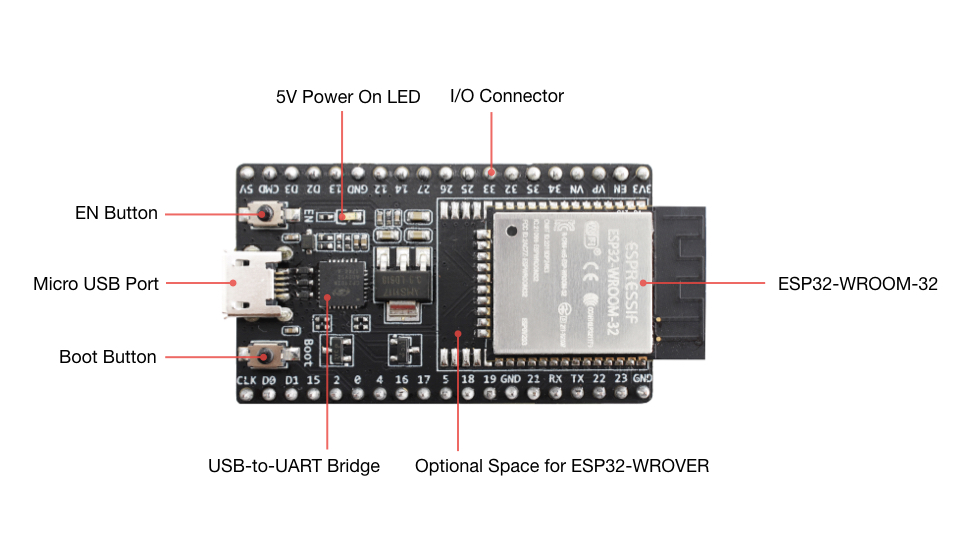
\includegraphics[scale=0.4]{images/esp32-devkitc.jpg}
        \caption{ESP32-DevKitC V4 with ESP32-WROOM-32 module \cite{esp32-gettingStarted_w}}
        \label{esp32_img}
    \end{figure}
\section{Choix de l'environnement}
    Trois environnements s'offrent à nous:
    \begin{enumerate}
        \item \textbf{MicroPython}\\
            Selon le site officiel de MicroPython\cite{micropython_w}, MicroPython est une implémentation simple et efficace de Python 3
            incluant un petit sous-ensemble de la bibliothèque standard Python et est optimisé pour fonctionner sur des microcontrôleurs.\\
            MicroPython est open source et facile à utiliser. Cependant, il n'est pas assez bas niveau pour ce projet.\\
            Par exemple il serait impossible d'envoyer des paquets au niveau de la couche lisaison de données ou encore, avoir accès aux tables de routages \textsc{ip}.\\
            %Nous n'utiliserons donc pas cet environnement.
        
        \item \textbf{IoT Development Framework (IDF)}\\
            IDF est l'environnement du constucteur de l'\esp\ (Espressif). La documentation est complète mais le code source n'est pas entièrement disponible. Pour certaines
            parties du framework, nous n'avons accès qu'aux fichiers d'entête.\\
            Ce framework est natif et nous apportera donc une plus grande fidélité à l'\esp. \\
            Cet environnement nous donne aussi accès à des fonctionnalités de FreeRTOS (free real-time operating system).\\
            FreeRTOS est un système d'exploitation temps réel open source pour microcontrôleurs. Ses fonctionnalités pourront nous être utiles pour le projet.\\

        \item \textbf{Arduino}\\
            L'environnement Arduino se base sur IDF. Il est donc possible que certaines fonctionnalités d'IDF ne soient pas disponible. La documentation est moins complète qu'IDF et tout le code source est disponible. Cet environnement semble assez bas
            niveau car nous avons accès au driver Ethernet et à la couche \textsc{ip}.
    \end{enumerate}

    Il est évident que nous ne choisirons pas MicroPython car certaines fonctionnalités utiles pour ce projet ne sont pas accessibles.\\
    Nous choisirons IDF pour sa documentation complète, sa nativité et l'accès aux fonctionnalités de FreeRTOS.
\section{Protocoles de routage}
    Dans cette section nous discuterons des différents protocoles de routage envisageables.\\
    Tout d'abord, nous établirons un classement des différents types de protocoles de routage \mesh. \\
    Ensuite, nous etudierons et comparerons différents protocoles de routage mesh: \espmesh\ \cite{esp-mesh_w}, OLSR\cite{olsr_w}, AODV\cite{aodv_w} et DSR\cite{dsr_w}\\
    Enfin nous pourrons choisir un protocole à implémenter sur \esp.\\
    
    \subsection{Classification}
    Les protocoles de routages \mesh\ peuvent être divisés en deux grandes catégories:
    \begin{enumerate}
        \item Proactifs: Les noeuds maintiennent une/des table(s) de routage
            qui stockent les routes vers tous les noeuds du réseau. 
            Ils envoient régulièrement des paquest de contrôle à travers le réseau pour échanger et 
            mettre à jour l'information de leurs voisins.
        \item Réactifs: Ces protocoles établissent une route uniquement quand des paquets
            doivent être transférés.
    \end{enumerate}
    Nous écarterons les protocoles proactifs pour se projet car ils gardent
    beaucoup d'information en mémoire. Ils ne passent donc pas à l'échelle.\\
    Les protocoles réactifs sont plus énconomes en ressources mais nécessitent parfois un délai plus long pour établir une route
    car elles sont établies à la demande.\\
    
    Ci-dessous, une brève classifications des protocoles de routages \mesh.
    \begin{diagram}[H]
        \Tree[.{wireless network protocols} [.Reactive [.\textsc{aodv} ][.\textsc{dsr} ]] [.Proactive [.{Link-state} [.\textsc{olsr} ] [.\textsc{b.a.t.m.a.n} ]] [.{Distance-vector} [.\textsc{dsdv} ]]]]
        \caption{Classifications des protocols de routage }
    \end{diagram}
    \begin{flushleft}
        \textbf{AODV} Ad-hoc On-demand Distance Vector\\
        \textbf{DSR} Dynamic Source Routing\\
        \textbf{OLSR} Optimized Link State Routing\\
        \textbf{B.T.M.A.N} Better Approach to Mobile Adhoc Networking\\
        \textbf{DSDV} Destination Sequence Distance Vector\\
    \end{flushleft}

    \subsection{Etude des différents protocoles}
    \subsubsection{\underline{ESP MESH}}%\underline{\textbf{ESP MESH}}\\
        \espmesh\ est le protocol du constructeur Espressif permettant d'établir un réseau mesh avec des \esp.
        Cette section explique le fonctionnement de ce protocole. La topologie utilisée ici est l'arbre.
        Il existe plusieurs types de noeuds:
        \begin{enumerate}
            \item Racine: Seule interface entre le réseau \espmesh\ et un réseau \textsc{ip} externe
            \item Noeuds intermédiaires: Noeuds qui ont un parent et au moins un enfant.
            Ils peuvent transmettre leurs paquets et ceux de leurs enfants.
            \item Feuilles: noeuds qui n'ont pas d'enfants et ne transmettent que leur paquets.
            \item Noeuds idle: noeuds qui n'ont pas encore rejoint un réseau \espmesh\ 
        \end{enumerate}

        \begin{figure}[H]
            \centering
            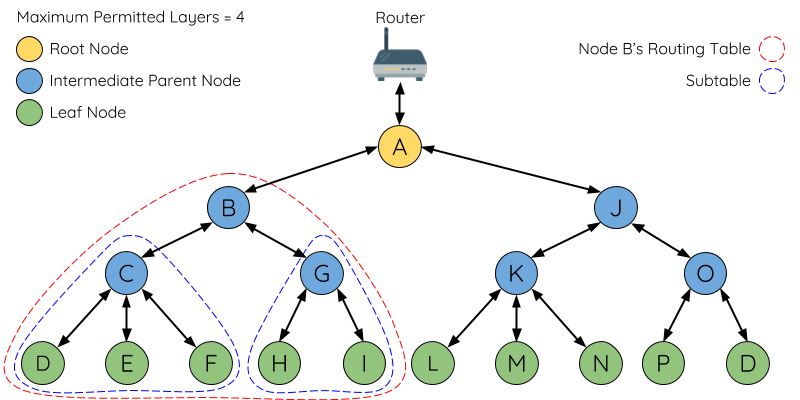
\includegraphics[scale=0.3]{images/mesh-node-types.png}
            \caption{Topologie d'un réseau \espmesh \cite{esp-mesh_w}}
        \end{figure}

        \textbf{Routage}\newline
        \begin{enumerate}
            \item Table de routage\\
                Chaque noeud possède sa table de routage. Soit $p$ un noeud, sa table de routage contient les addresses \mac\ 
                des noeuds du sous-arbre ayant $p$ comme racine, et également celle de $p$.\\
                Elle est partitionnée en sous-tables qui correspondent au sous-arbres des enfants de $p$.
            \item Acheminement de paquets\\
                Quand un paquet est reçu,
                \begin{itemize}
                    \item Si l'adresse \mac\ du paquet est dans la table de routage et si elle est différente de l'adresse du noeud l'ayant reçu, le paquet est envoyé
                    à l'enfant correspondant à la sous-table contenant l'adresse.
                    \item Si l'adresse n'est pas dans la table de routage, le paquet est envoyé au parent.
                \end{itemize}
                %\espmesh\ utilise un mécanisme de vérification de chemin pour détecter les boucles. Si une boucle arrive, un parent va prévenir son enfant et initier une déconnexion.

        \end{enumerate}
        \vspace{0.5cm}

        \textbf{Construction d'un réseau}
        \newline
        \begin{enumerate}
            \item \'Election de la racine
                \begin{itemize}
                    \item \textbf{Sélection automatique}\\
                        Chaque noeud se trouvant à l'état idle va transmettre son addresse \mac\ et
                        la valeur de son \rssi\ (Received Signal Strength Indication) avec le routeur via des beacons.\\
                        Simultanément, chaque noeud scanne les beacons des autres noeuds. Si un noeud
                        en détecte un autre avec un \rssi\ strictement plus fort, il va transmettre le contenu de
                        ce beacon (càd voter pour ce noeud).\\
                        Ce processus sera répété pendant un nombre minimum d'itérations.\\
                        Après toutes les itérations, chaque noeud va calculer le ratio
                        \[\frac{nombre\ de\ votes}{nombre\ de\ noeuds\ participants\ \textrm{\textit{à l'élection}}}\]
                        Si ce ratio est au dessus d'un certain seuil (par défaut 90\%), ce noeud deviendra la racine.\footnote{
                            Si plusieurs racines sont élues, deux réseaux \espmesh\ seront créés.
                            Dans ce cas, \espmesh\ possède un mécanisme interne qui va fusionner les deux réseaux
                            ssi les racines sont connectées au même routeur.
                        }



                    \item \textbf{Sélection par l'utilisateur}\\
                        La racine se connecte au routeur et elle ainsi que les autres noeuds, oublient le processus
                        d'élection.
                \end{itemize}
            \item Formation de la deuxième couche\\
                Une fois le processus d'élection d'une racine terminé, chaque noeuds va émettre des beacons
                pour permettre aux autres noeuds de détecter sa présence et de connaître son status.
                Ces beacons contiennent les informations suivantes:
                \begin{itemize}
                    \item[$\bullet$] Type du noeud (racine, intermédiaire, feuille, idle)
                    \item[$\bullet$] Couche sur laquelle se trouve le noeud
                    \item[$\bullet$] Nombre de couches maximum autorisées dans le réseau
                    \item[$\bullet$] Nombre de noeuds enfants
                    \item[$\bullet$] Nombre maximum d'enfants   
                \end{itemize}
                Les noeuds idle à portée de la racine vont s'y connecter et devenir des noeuds intermédiaires.
            
            \item Formation des autres couches\\
                Les noeuds idle à portée de noeuds intermédiaires vont s'y connecter. Si plusieurs parents
                sont possibles, un noeud choisira son parent selon deux critères connus par les beacons des noeuds intermédiaires.
                \begin{enumerate}
                    \addtolength{\itemindent}{1cm}
                    \item[1.] La couche sur laquelle se situe le candidat parent:
                        le candidat se trouvant sur la couche la moins profonde sera choisi. 
                    \item[2.] Le nombre d'enfants du candidat parent: si plusieurs candidats se trouvent
                        sur la couche la moins profonde, celui avec le moins d'enfants sera choisi. 
                \end{enumerate}
                
                Un noeud peut aussi se connecter à un parent prédéfini.\\

                Une fois connectés, les noeuds deviennent des noeuds intermédiaires si le nombre maximal de couches n'est pas atteint.
                Sinon, les noeuds de la dernière couche deviennent automatiquement
                des feuilles, empêchant d'autres noeuds dans l'état idle de s'y connecter.

        \end{enumerate}
        Pour éviter les boucles, un noeud ne va pas se connecter à un noeud dont l'adresse \mac\ se trouve dans sa table de routage.
        \vspace{0.5cm}

        \textbf{Mise sous tension asynchrone}\newline
            La structure du réseau peut être affectée par l'ordre dans lequel les noeuds sont mis sous tension.
            Les noeuds ayant une mise en tension retardée suivront les deux règles suivantes:
            \begin{enumerate}
                \item Si une racine existe déja, le noeud ne vas pas essayer d'élire une nouvelle racine
                    même si son \rssi\ avec le routeur est meilleur. Il va rejoindre le réseau comme un noeud idle. \\
                    Si le noeud est la racine désignée, tous les autres noeuds vont rester dans l'état idle
                    jusqu'a ce que le noeud soit mis sous tension.
                \item Si le noeud devient un noeud intermédiraire, il peut devenir le meilleur parent d'un autre noeud ( cet autre noeud changera donc de parent).
                \item Si un noeud idle a un parent prédéfini et que ce noeud n'est pas sous tension, il ne vas pas essayer de se connecter à un autre parent.
            \end{enumerate}
        \vspace{0.5cm}
        \textbf{Défaillance d'un noeud}\newline
            \begin{itemize}
                \item Défaillance de la racine\\
                    Si la racine tombe, les noeuds de la deuxième couche vont d'abord tenter de s'y reconnecter.
                    Après plusieurs échecs, les noeuds de la deuxième couche vont entamer entre eux, le processus d'élection d'une nouvelle racine.\\
                    Si la racine ainsi que plusieurs couches tombent, le processus d'élection sera initialisé sur la couche la plus haute.


                \item Défaillance d'un noeud intermédiaire\\
                    Si un noeud intermédiaire tombe, ses enfants vont d'abord tenter de s'y reconnecter.
                    Après plusieurs échecs, ils se connecteront au meilleur parent disponible.\\
                    S'il n'y a aucun parent possible, ils se mettront dans l'état idle.
                    \begin{figure}[H]
                        \centering
                        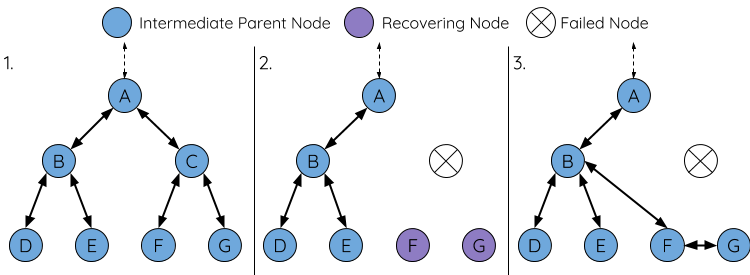
\includegraphics[scale=0.5]{images/mesh-parent-node-failure.png}
                        \caption{Défaillance d'un noeud intermédiaire\cite{esp-mesh_w}}
                    \end{figure}
            \end{itemize}
            \vspace{0.5cm}
            \textbf{Changement de racine}\newline
                Un changement de racine n'est possible que dans deux situations:
                \begin{enumerate}
                    \item La racine tombe. (voir point précédent)
                    \item La racine le demande.
                        Dans ce cas, un processus d'élection de racine sera initialisé. La nouvelle racine élue
                        enverra alors une switch request à la racine actuelle qui répondra par un acquittement.
                        Ensuite la nouvelle racine se déconnectera de son parent et se connectera au routeur.
                        L'ancienne racine se déconnectera du routeur et rentrera dans l'état idle pour enfin se connecter à un nouveau parent.
                \end{enumerate}
        \textbf{Paquets ESP-MESH}\\
            Les paquets \espmesh\ sont contenus dans une trame wifi. Une transmission multi-sauts utilisera un paquet \espmesh\ transporté entre chaque noeuds par un paquet wifi différent.\\
            La figure \ref{fig_meshPacket} montre la structure d'un paquet \espmesh:\\

            \begin{figure}[h]
                \centering
                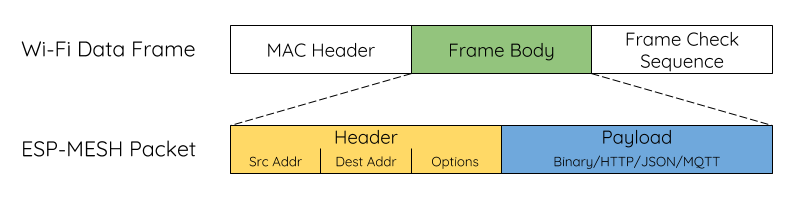
\includegraphics[scale=0.5]{images/mesh-packet.png}
                \caption{Paquet \espmesh\ \cite{esp-mesh_w}}
                \label{fig_meshPacket}
            \end{figure}
            Le header d'un paquet \espmesh\ contient les adresses \mac\ source et destination ainsi que diverse options.\\
            Le payload d'un paquet \espmesh\ contient les données de l'application.
        
        \vspace{0.5cm}
        \textbf{Multicasting}\\
            Le multicasting permet d'envoyer simultanément un paquet \espmesh\ à plusieurs noeud du réseau. Le multicasting
            peut être réalisé en spécifiant
            \begin{itemize}
                \item Soit un ensemble d'adresses \mac\\
                    Dans ce cas, l'adresse de destination doit être
                    {\fontfamily{qcr}\selectfont \textls[-300]{\small 0 1 : 0 0 : 5 E : x x : x x : x x}}
                    Cela signifie que le paquet est un paquet multicast et que la liste des adresses peut être obtenue dans les options du header.
                \item Soit un groupe préconfiguré de noeuds\\
                    Dans ce cas, l'adresse de destination du paquet doit être l'ID\footnote{Dans un réseau\espmesh, chaque groupe a un ID unique}
                    du groupe et un flag \textsc{mesh\_data\_group} doit être ajouté. % todo ajouté où ?
                    % todo comment les noeuds sont au courant qu'ils sont dans ce groupe
            \end{itemize}

        \vspace{0.5cm}
        \textbf{Broadcasting}\\
            Le broadcasting permet de transmettre un paquet \espmesh\ à tous les noeuds du réseau. Pour éviter de gaspiller de
            la bande passante, \espmesh utilise les règles suivantes:
            \begin{enumerate}
                \item Quand un noeud intermédiare reçoit un paquet broadcast de son parent, il va le transmettre à tous ses enfants
                    et en stocker une copie
                \item Quand un noeud intermédiaire est la source d'un paquet broadcast, il va le transmettre à son parent et à ses enfants
                \item Quand un noeud intermédiaire reçoit un paquet d'un de ses enfants, il va le transmettre à ses autres enfants, son parent
                    et en stocker une copie
                \item Quand une feuille est la source d'un paquet broadcast, elle va le transmettre à son parent
                \item Quand la racine est la source d'un paquet broadcast, elle va le transmettre à ses enfants
                \item Quand la racine reçoit un paquet broadcast de l'un de ses enfants, elle va le transmettre à ses autres enfants et en stocker une copie
                \item Quand un noeud reçoit un paquet broadcast avec son addresse \mac\ comme adresse source, il l'ignore
                \item Quand un noeud intermédiaire reçoit un paquet broadcast de son parent, s'il possède une copie de ce paquet (càd que ce paquet a été à l'origine transmis par l'un de ses enfants), il va l'ignorer
                    pour éviter les cycles ( protocole d'inondation)
            \end{enumerate}
        \vspace{0.5cm}
        \textbf{Contrôle de flux}\\%todo pas clair
            Pour éviter que les parents soient submergés de flux venant de leurs enfants, chaque parent va
            assigner une fenêtre de réception à chaque enfant. Chaque noeud enfant doit demander une fenêtre
            de réception avant chaque transmission. La taille de la fenêtre peut être ajustée dynamiquement.
            Une transmission d'un enfant vers un parent se déroule en plusieurs étapes:
            \begin{enumerate}
                \item Le noeud enfant envoit à son parent une requête de fenêtre. Cette requête contient le numéro de séquence du paquet en attente d'envoi.
                \item Le parent reçoit la requête et compare le numéro de séquence avec celui du précédent paquet envoyé par l'enfant.
                    La comparaison est utilisée pour calculer la taille de la fenêtre qui est transmise à l'enfant.
                \item L'enfant transmet le paquet en accord avec la taille de fenêtre. Une fois la fenêtre de réception utilisée, l'enfant doit renvoyer une demande de fenêtre.
            \end{enumerate}
        \vspace{0.5cm}
        \textbf{Performances}\\
            Espressif fournit les performances d'\espmesh\ pour un réseau de 100 noeuds avec un nombre maximum de couches de 6 
            et un nombre d'enfants maximum par noeuds de 6.(voir table \ref{performances_espMesh})
            \begin{table}[H]
                \begin{tabular}{|l|l|}
                    \hline
                    Temps de construction du réseau & $<$ 60 secondes\\ \hline
                    Latence par saut & 10 à 30 millisecondes\\ \hline
                    Temps de réparation du réseau & \makecell{Si la racine tombe: $<$ 10 secondes \\ Si un noeud enfant tombe: $<$ 5 secondes}\\ \hline
                \end{tabular}
                \caption{Performances d'\espmesh\ \cite{esp-mesh_w}}
                \label{performances_espMesh}
            \end{table}

            
        \textbf{Discussion}\\
            A première vue, une topologie en arbre n'est pas robuste car si la racine tombe,
            tout le reste du réseau est déconnecté. Cependant le processus d'élection
            d'une nouvelle racine semble efficace selon les résulats fournis par Espressif.
            Un point négatif du protocole est que les tables de routage contiennent tous le sous arbre des noeuds.
            On imagine donc difficilement utiliser ce protocole pour un nombre élevé de noeuds.
    

    \vspace{2cm}
    \subsubsection{\underline{OLSR}}%\underline{\textbf{OLSR}}\\ ##########################
    %##########################################################################
        \textit{OLSR} est un protocole proactif à état de liens. Il fournit un support à certaines extensions comme
        sleep mode operation, multicast-routing etc.\\
        Ce protocole utilise deux types de messages:\\
        \begin{enumerate}
            \item \textit{hello}\\
                Ces paquets sont envoyés à un saut. Ils sont utilisés pour constituer le voisinage et
                l'ensemble des \textit{"multipoint relays" (MPR)}. (concept expliqué  \hyperlink{mpr}{ici})\\
                Ils contiennent le status des liens d'un noeud avec tout son voisinage.
            \item \textit{topology control (TC)}\\
                Diffusés dans tous le réseau par les \textit{MPR}. Ils contiennt la liste de tous les \textit{MPRs}
                du noeud qui émet ce paquet.
        \end{enumerate}
        \hypertarget{mpr}{\textit{\textbf{MPR}}}\\
        Les multipoint relays sont des noeuds qui sont chargés d'effectuer le broadcasting des \textit{TCs}. \\
        L'ensemble des \textit{MPRs} d'un réseau \textit{OLSR} forme un arbre couvrant du réseau. Trouver ce sous-ensemble de sommets
        est un problème \textit{NP-Complet}. \textit{DSR} propose une heursitique simple pour calculer cet ensemble de \textit{MPRs}.\\
        
        \begin{figure}[H]
            \centering
            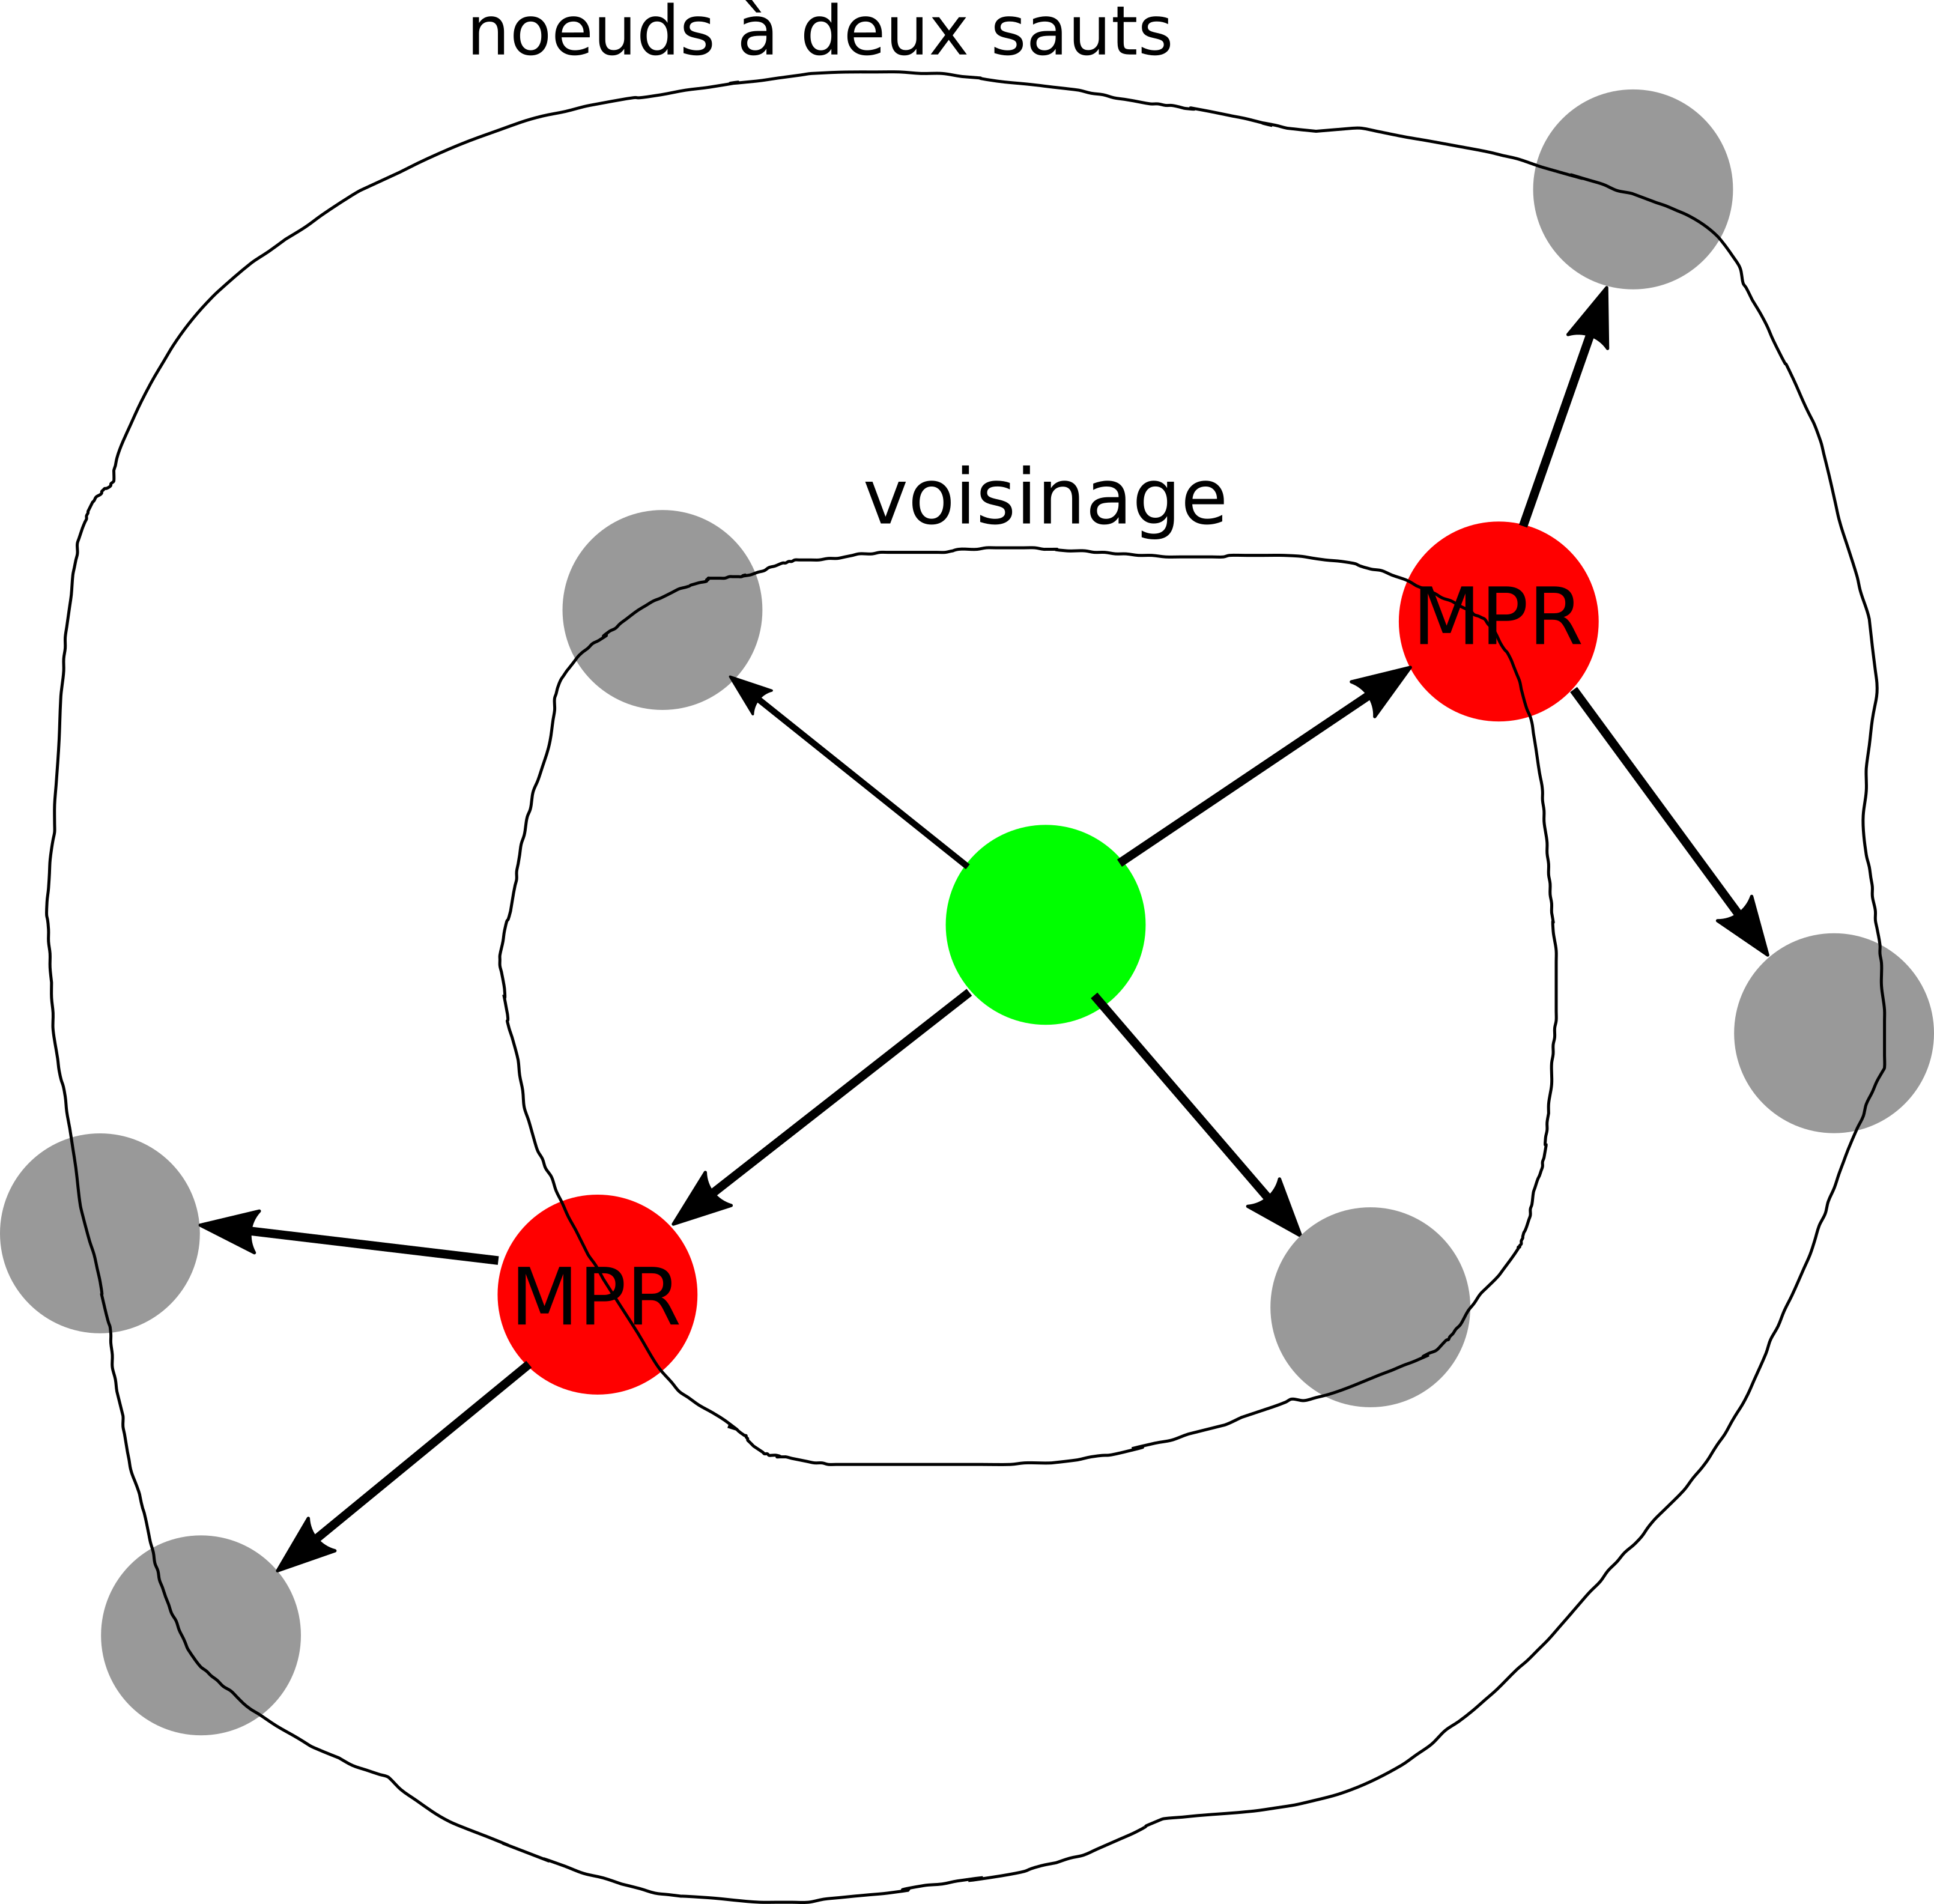
\includegraphics[scale=0.5]{images/olsr.png}
            \caption{Shéma d'un réseau OLSR}
            \label{olsr}
        \end{figure}

        \textbf{Découverte de voisins}\\
        La découverte de voisins se fait comme suit:
        \begin{itemize}
            \item Quand un noeud B reçoit un message \textit{hello} d'un noeud A,
                il va rajouter A dans ses voisins avec le status \underline{asymétrique}
            \item B va ensuite envoyer un message \textit{hello} avec A asymétrique dans la liste de voisins.
            \item Quand a reçoit se message, il va pouvoir modifier le statut de B à symétrique.
            \item A renvoie un message \textit{hello} avec B symétrique dans la liste des voisins.
            \item Quand B reçoit ce message il modifie le statut de A à symétrique
        \end{itemize}
        \begin{figure}[H]
            \centering
            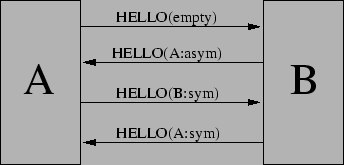
\includegraphics[scale=0.6]{images/olsr_neighborDiscovery.png}
            \caption{découverte de voisins en utilisant les messages \textit{hello} \cite{olsr_neighborDiscovery_w}}
            \label{olsr_neighborDiscovery}
        \end{figure}
    
    \subsubsection{\underline{AODV}}%\underline{\textbf{AODV}}\\
        Ad-hoc On-demand Distance Vector (AODV) est un protocole réactif à vecteur de distance.\\
        Ce protocole définis 3 types de messages:
        \begin{enumerate}
            \item Route request (\textit{RREQs})
            \item Route Remplies (\textit{RREPs})
            \item Route Errors (\textit{RERRs})
        \end{enumerate}

        
        \underline{\textbf{Format des paquets}}\\
        
        
        \textbf{RREQ}
        \begin{figure}[H]
        \centering
            \begin{verbatimtab}
 0                   1                   2                   3
 0 1 2 3 4 5 6 7 8 9 0 1 2 3 4 5 6 7 8 9 0 1 2 3 4 5 6 7 8 9 0 1
+-+-+-+-+-+-+-+-+-+-+-+-+-+-+-+-+-+-+-+-+-+-+-+-+-+-+-+-+-+-+-+-+
|     Type      |J|R|G|D|U|   Reserved          |   Hop Count   |
+-+-+-+-+-+-+-+-+-+-+-+-+-+-+-+-+-+-+-+-+-+-+-+-+-+-+-+-+-+-+-+-+
|                            RREQ ID                            |
+-+-+-+-+-+-+-+-+-+-+-+-+-+-+-+-+-+-+-+-+-+-+-+-+-+-+-+-+-+-+-+-+
|                    Destination IP Address                     |
+-+-+-+-+-+-+-+-+-+-+-+-+-+-+-+-+-+-+-+-+-+-+-+-+-+-+-+-+-+-+-+-+
|                  Destination Sequence Number                  |
+-+-+-+-+-+-+-+-+-+-+-+-+-+-+-+-+-+-+-+-+-+-+-+-+-+-+-+-+-+-+-+-+
|                    Originator IP Address                      |
+-+-+-+-+-+-+-+-+-+-+-+-+-+-+-+-+-+-+-+-+-+-+-+-+-+-+-+-+-+-+-+-+
|                  Originator Sequence Number                   |
+-+-+-+-+-+-+-+-+-+-+-+-+-+-+-+-+-+-+-+-+-+-+-+-+-+-+-+-+-+-+-+-+
            \end{verbatimtab}
        \caption{format d'un paquet RREQ \cite{aodv_w}}
        \label{rreqPaquet}
    \end{figure}

    Où J,R,G,D,U sont des flags.\\
        
        \textbf{RREP}
        \begin{figure}[H]
            \centering
                \begin{verbatimtab}
 0                   1                   2                   3
 0 1 2 3 4 5 6 7 8 9 0 1 2 3 4 5 6 7 8 9 0 1 2 3 4 5 6 7 8 9 0 1
+-+-+-+-+-+-+-+-+-+-+-+-+-+-+-+-+-+-+-+-+-+-+-+-+-+-+-+-+-+-+-+-+
|     Type      |R|A|    Reserved     |Prefix Sz|   Hop Count   |
+-+-+-+-+-+-+-+-+-+-+-+-+-+-+-+-+-+-+-+-+-+-+-+-+-+-+-+-+-+-+-+-+
|                     Destination IP address                    |
+-+-+-+-+-+-+-+-+-+-+-+-+-+-+-+-+-+-+-+-+-+-+-+-+-+-+-+-+-+-+-+-+
|                  Destination Sequence Number                  |
+-+-+-+-+-+-+-+-+-+-+-+-+-+-+-+-+-+-+-+-+-+-+-+-+-+-+-+-+-+-+-+-+
|                    Originator IP address                      |
+-+-+-+-+-+-+-+-+-+-+-+-+-+-+-+-+-+-+-+-+-+-+-+-+-+-+-+-+-+-+-+-+
|                           Lifetime                            |
+-+-+-+-+-+-+-+-+-+-+-+-+-+-+-+-+-+-+-+-+-+-+-+-+-+-+-+-+-+-+-+-+
                \end{verbatimtab}
            \caption{format d'un paquet RREP \cite{aodv_w}}
            \label{rreqPaquet}
        \end{figure}

        Où R et A sont des flags.\\

        \underline{\textbf{Découverte d'un chemin}}\\
        La découverte de chemin est intiée par un noeud voulant envoyer des paquets à une desination pour laquelle il n'a aucune information.\\
        Chaque noeud possède deux compteurs: \textbf{\textit{sequence\_number}} et \textbf{\textit{rreq\_id}}.\\
        
        \textbf{Génération du \textit{RREQ}}\\
            Le noeud source incrémente ses compteurs \textbf{\textit{sequence\_number}} et \textbf{\textit{rreq\_id}} de 1.
            Il envoie ensuite un \textit{RREQ} en broadcast à ses voisins.\\
        
            \textbf{Propagation du \textit{RREQ}}\\
        \begin{itemize}
            \item[$\bullet$] \underline{Noeud intermédiaire}\\
                A la réception d'un \textit{RREQ}, un noeud intermédiaire va pouvoir rajouter ou mettre à jour
                les routes vers le noeud source du \textit{RREQ} et vers son prédécesseur.\\
                Ensuite deux situations sont possibles:
                \begin{enumerate}
                    \item Le noeud courant possède une route active vers la destination et le numéro de séquenc de la route est plus grand ou égale au numéro de séquence
                        de la desination dans le \textit{RREQ}.\\
                        Dans ce cas il peut envoyer par unicast un \textit{RREP} à la source du \textit{RREQ}
                    \item La condition en 1. n'est pas satisfaite.\\
                        Dans ce cas, le noeud va incrémenter le nombre de sauts du \textit{RREQ} et le propager à ses voisins.\\
                \end{enumerate}
                

            \item[$\bullet$] \underline{Noeud destination}\\
                A la réception d'un \textit{RREQ} lui étant destiné, un noeud va, comme un noeud intermédiaire, 
                rajouter ou mettre à jour les routes vers le noeud source du \textit{RREQ} et vers son prédécesseur.\\
                Si le \textbf{\textit{Destination Sequence Number}} du \textit{RREQ} est égale à son \textbf{\textit{sequence\_number}},
                il va incrémenter ce dernier et envoyer un \textit{RREP} en unicast vers la source du \textit{RREQ}.\\
             
        \end{itemize}


        \textbf{Propagation du \textit{RREP}}\\
            A la réception d'un \textit{RREP}, un noeud va pouvoir rajouter ou mettre à jour
            les routes vers le noeud source du \textit{RREP} et vers son sucesseur.\\
            Il va ensuite incrémenter le nombre de sauts du \textit{RREP} et le propager en unicast vers la destination de ce \textit{RREP}.\\

        \underline{\textbf{Table de routage}}\\
        
        Chaque entrée d'une table de routage contient les informations suivantes:
        
        \begin{table}[H]
            \centering
            \begin{tabular}{|l|l|}
                \hline
                \textit{dest}       & Adresse IP de destination\\
                \textit{dest\_SN}   & Numéro de séquence de destination\\
                \textit{flag}       & Indicateur de numéro de séquence de destination valide\\
                \textit{out}        & Interface réseau\\
                \textit{hops}       & Comptage du saut (nombre de sauts nécessaires pour atteindre la destination)\\
                \textit{next-hop}   & Prochain saut\\
                \textit{precursors} & Liste des précurseurs\\
                \textit{lifetime}   & temps d'expiration ou de suppression de l'itinéraire\\
                \hline
            \end{tabular}
            \caption{entrée d'une table de routage \aodv \cite{aodv_w}}
            \label{routingTable_aodv}
        \end{table}

        \textbf{Mise à jour de la table de routage}\\
            Soit N une nouvelle route et O la route existante.\\
            O est mise à jour si:\\
            \begin{center}
                \begin{tabular}{|l|}
                    \hline
                    $O.SN \leq N.SN$ \\
                    \textbf{ou} ($O.SN = N.SN$ \textbf{et} $O.hop\_count > N.hop\_count$)\\
                    \hline
                \end{tabular}
            \end{center}
        
        \textbf{Gestion du \textit{lifetime}}\\
            Le temps de vie d'une route dans la table de routage est initialisé à \textit{active\_route\_timeout} (3 millisecondes).\\
            Quand ce timer expire, la route passe de active à inactive. Une route inactive ne pourra plus être utilisée pour transférer des données
            mais pourra fournir des informations pour de futurs \textit{RREQ} et la réparation de routes.\\
            Quand une route est utilisée, son temps de vie  est actualisé à: $current time + active\_route\_timeout$


        \underline{\textbf{Evitement de boucles}}\\
            A priori les numéros de séquences suffisent pour éviter les boucles. Cependant, d'après \cite{loop_aodv_w}, il y a des
            ambiguités dans le RFC \cite{aodv_w}. Certaines parties du RFC concerant la gestion des numéros de séquences pourraient introduire
            des boucles. Nous approfondirons la lecture de cet article si nous choisissons ce protocole afin d'éviter les boucles dans notre implémentation.

    \subsubsection{\underline{DSR}}%\underline{\textbf{DSR}}\\
        Comme \textit{AODV}, \textit{DSR} est un protocole réactif à vecteur de distance.\\
        % ack lors de la reception d'un paquet
        Deux mécanismes principaux caractérisent \textit{DSR}\\
        \begin{enumerate}
            \item \textbf{Route Discovery}\\
                Similaire à la découverte de chemins dans AODV. La différence est que le \textit{RREQ} va contenit l'id de tous les sauts de chemin.\\
                Quand la cible d'un \textit{RREQ} le reçoit, elle va répondre avec un \textit{RREP} contenant le chemin du \textit{RREQ} inversé.\\
                Quand des paquets de données contiennent le chemin complet par lequel ils doivent transiter.\\
                On a donc des paquets d'une taille variant avec celle du chemin emprunté.
            \item \textbf{Route Maintenance}\\
                Chaque noeud est résposables des liens entre lui et ses sucesseurs et possède une cache de routes.
                Pour cela, quand un noeud reçoit un paquet, il va transmettre à la source de ce paquet
                un ack. Si le ack n'est pas reçu au bout d'un temps fixé, l'émetteur du paquet va émettre
                un paquet \textit{route\_error} à ses prédécesseurs pour leur signaler que le lien n'existe plus.\\
                Si des routes sont interrompues, les noeuds peuvent soit utiliser d'autres routes de leur cache, soit initier une \textit{route discovery}

        \end{enumerate}
        \begin{figure}[H]
            \centering
            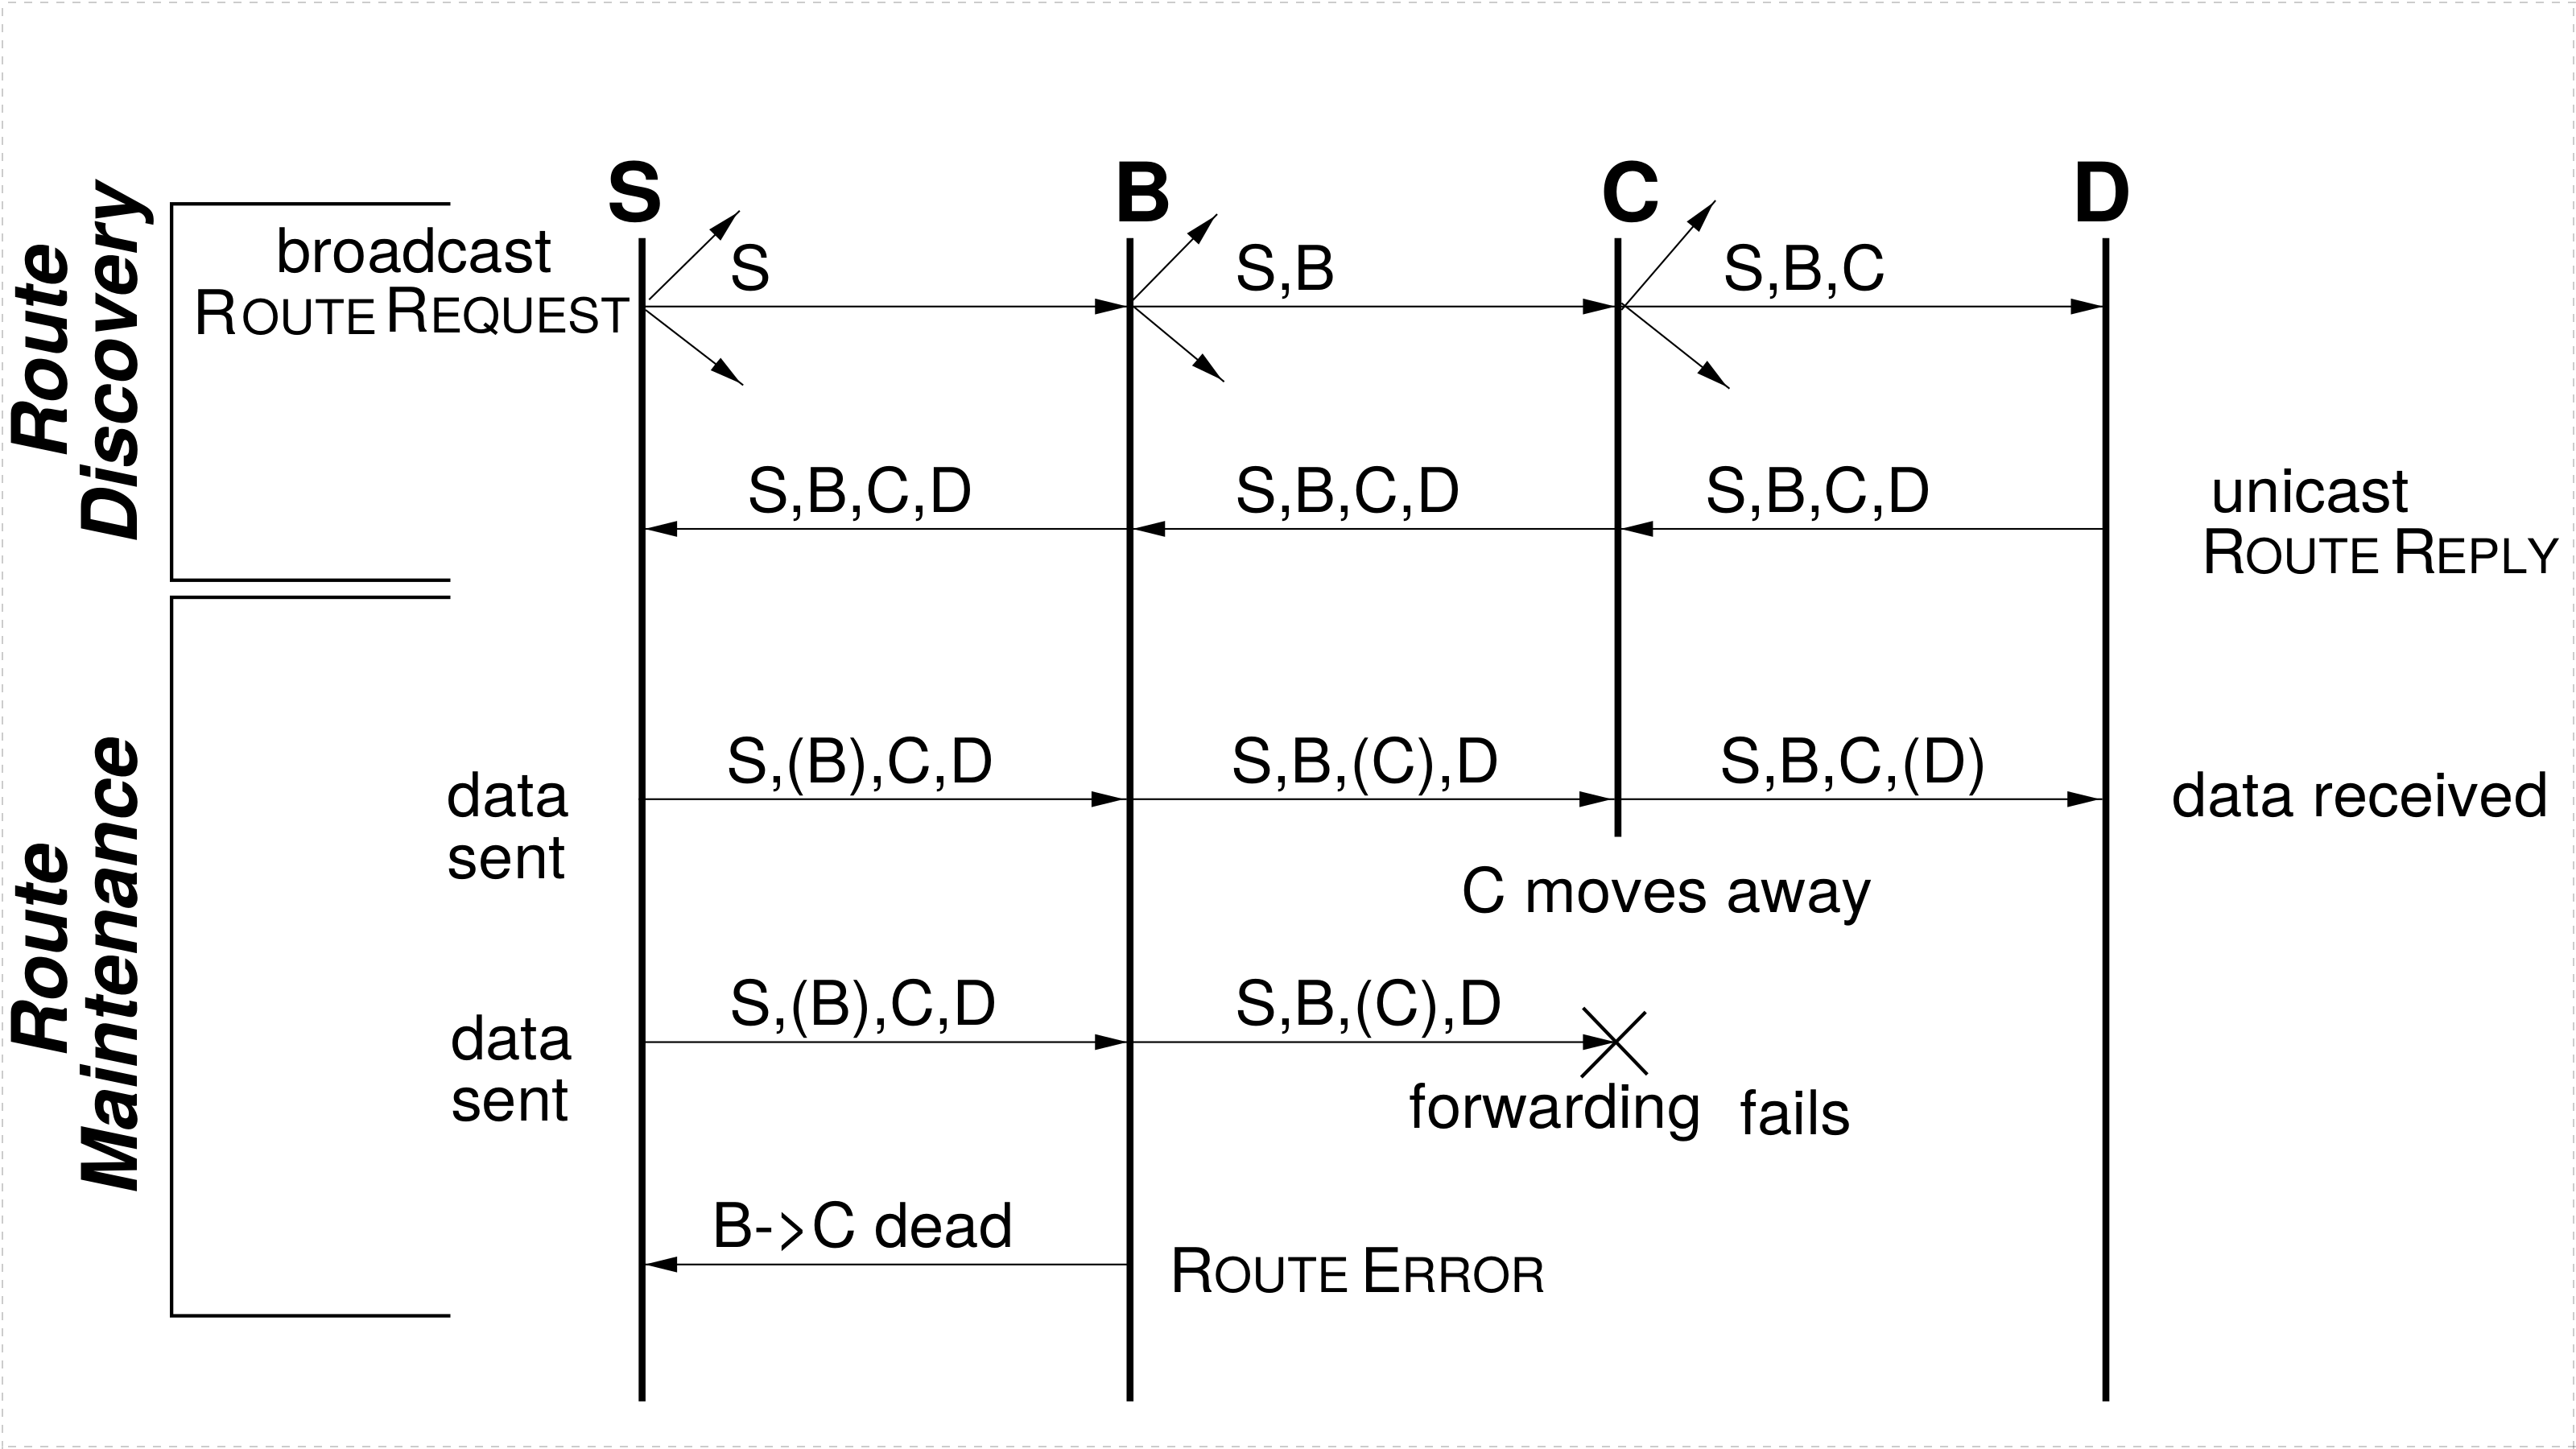
\includegraphics[scale=0.12]{images/ack_dsr.png}
            \caption{Illustration de DSR \cite{dsr_for_adHoc_network}}
            \label{dsr_image}
        \end{figure}
\chapter{Implémentation}
\section{Limitations}
        Le driver Wi-Fi d'\textit{IDF} ne nous permet pas d'avoir une connection
        avec plusieurs noeud simultanément. \espnow\ pourraît être une solution
        pour palier à ce problème.\\
    
    
        \textbf{ESP NOW}\\
            \espnow\ est un protocole de communication Wi-Fi sans connexion définis par Espressif.\\
            Nous n'avons trouvé aucune documentation décivant le fonctionnement de ce protocole.\\
            Avec la documentation disponible, nous savons qu'un noeud a une liste de \textit{peers} (ses voisins) avec qui il peut échanger des données.
            Le nombre de voisins est limité à 20. Cette limite ne posera pas problème pour ce projet.
        

\section{Prochaines étapes}
        \begin{enumerate}
            \item Nous allons créer un réseau \espmesh. Ceci nous permettra de nous
            familiariser avec l'environnement \textit{IDF}.
            \item Nous évaluerons les performances et fonctionnalités de ce protocole.
            \item Nous implémenterons un protocole de routage mesh choisis plus haut.
            \item L'objectif est de l'implémenter au niveau de la couche liaison de données.
                Si nous rencontrons trop de difficulté ou que nous jugeons que ce choix n'est pas judicieux,
                nous implémenterons ce protocole au niveau de la couche réseau.
            \item Nous évaluerons les performances et fonctionnalités du prorotype créé. 
            
        \end{enumerate}

%\listoffigures
\bibliography{biblio.bib}{}
\bibliographystyle{plain}

\end{document}